\chapter{AWS Glue Scanner}

The previous chapters were devoted to Embedded Code Service. In this chapter, we will cover the details of the development of AWS Glue scanner prototype. AWS Glue is one of the data technologies that uses embedded code, so we will see how Embedded Code Service service can be used in data lineage analysis. To begin, we will describe AWS Glue and discuss it in terms of data lineage analysis. Next, we discuss and justify the design of a minimum viable product (MVP) of AWS Glue  scanner. Finally, we will look at its implementation. 

%%----- SECTION -----%%
\section{Motivation}

We have already briefly introduced AWS Glue in Section~\ref{sec:sourceTechnologyAnalysis}. Before we dive deeper into its analysis, we shall explain why we picked AWS Glue to demonstrate Embedded Code Service capabilities.
\par
The decision to implement Embedded Code Service in Manta Flow was motivated by the demand to analyze embedded code in several data technologies. Out of the existing programming language scanners in Manta Flow, Python scanner seemed to be the most prospective one to offer attractive value to customers for two reasons: it is widely used and the scanner yielded promising data lineage results.
\par
At this point, there were two options for selecting the data technology for MVP implementation. We could either choose an already supported one that uses embedded Python code to extend its capabilities, or create a new scanner for an unsupported data technology. For the first option, we could choose SAS, but there was no demand for such feature as Python support has only recently been added into it. For the second option, there have long been plans for AWS Glue and Databricks scanners based on customer demand, both of which use Python extensively. Out of these two, AWS Glue uses Python in a more straight-forward way as AWS Glue jobs are in fact complete Python scripts, which was close to what Python scanner could already analyze with limited results.

\section{AWS Glue analysis}

Before we can start designing the scanner, we need to analyze how AWS Glue works, how it processes data, what metadata it stores and how we can read it etc. 

\subsection{Overview}

AWS Glue is a cloud-based data integration service for discovering, cataloging and transforming data. It is a \textit{serverless} service, which means that there is no dedicated server which requires setup or maintenance. Each execution is managed by AWS Glue which allocates computing capacity on the machines present in a data center, executes the task and then frees the resources for any other task. The customer does not need to perform any maintenance, they only pay for used computing capacity and instead may focus on developing their data processes.
\par
AWS Glue provides its users with several key features:
\begin{enumerate}
    \item \textbf{Data Catalog}: AWS Glue includes a centralized metadata repository, known as Data Catalog. It stores metadata information about the data sources, tables, and schemas, making it easier to discover and understand the available data.
    \item \textbf{ETL jobs}: AWS Glue allows users to define and run ETL jobs using a visual interface or by writing custom code. ETL jobs enable data transformations such as filtering, aggregating, and joining data from different sources.
    \item \textbf{Data crawling}: AWS Glue can automatically discover and catalog data from various sources, including databases, data lakes, and file systems. It uses crawlers to scan the data sources, infer schemas, and create tables in the Data Catalog.
    \item \textbf{Data preparation}: AWS Glue provides capabilities for cleaning and preparing data before it is used for analysis. It offers built-in transformations and mappings to standardize and transform data, as well as options for creating custom transformations using Python or Scala.
    \item \textbf{Integration with other AWS services}: AWS Glue integrates with other AWS services, such as Amazon S3, Amazon Redshift, and Amazon Athena, allowing users to seamlessly move and transform data between these AWS services.
\end{enumerate}
\par
These features are split into two modules: \textit{Data Integration and ETL} and \textit{Data Catalog}.

\subsubsection{Data Integration and ETL}
The core of data integration in AWS Glue are ETL jobs executed on Apache Spark. Apache Spark is an open-source, distributed computing system that enables fast and flexible processing and analysis of large-scale data sets. It utilizes in-memory computing to accelerate iterative computations, making it ideal for big data workloads. With its distributed architecture, Spark can seamlessly distribute data and processing tasks across a cluster of computers, enabling parallel execution and efficient resource utilization. Spark provides a rich set of libraries and APIs for various data processing tasks available in several programming languages including Python and Scala.
\par
AWS Glue ETL jobs always contain a job script written in Python or Scala which is executed on Spark cluster configured in AWS Glue. Besides writing your own code, AWS Glue provides a tool with graphical user interface for creating ETL jobs. They can be created using transformations and data sources from the tool's toolbox. The tool auto-generates Python script based on the visualization. This script code can then be authored, but after that it can no longer be modified in the graphical tool.
We can see an example of an ETL job created in this tool in Figure~\ref{fig:visualJob}. This job reads a table from Data Catalog, renames some of the columns and filters out others and stores the result in a JSON file on Amazon S3, creating a Catalog table for it. Figure~\ref{fig:visualScript} shows the code generated by the tool and illustrates how ETL jobs written in Python look like.
\par
Another part of data integration is a scheduler for running jobs periodically or on custom triggers. The jobs can also be organized in a \textit{Workflow}, which is a different form of scheduling where multiple jobs can be executed in the order defined in the Workflow including various conditions and triggers.

\begin{figure}[ht]\centering
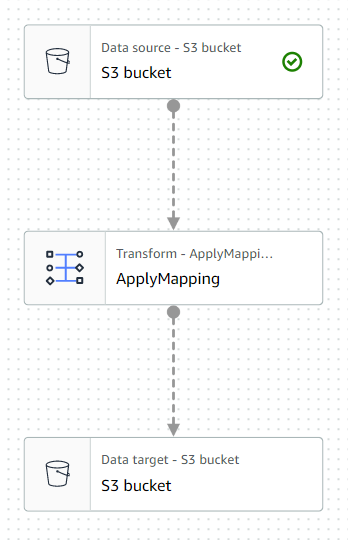
\includegraphics[height=0.6\textwidth]{img/job_example_visualization.png}
\caption{An example of an ETL job created in the graphical tool of AWS Glue}
\label{fig:visualJob}
\end{figure}

\begin{lstlisting}[language=Python,caption=Code script generated in AWS Glue for the ETL job created in a visual tool shown in Figure~\ref{fig:visualJob},label=fig:visualScript]
import sys
from awsglue.transforms import *
from awsglue.utils import getResolvedOptions
from pyspark.context import SparkContext
from awsglue.context import GlueContext
from awsglue.job import Job

args = getResolvedOptions(sys.argv, ["JOB_NAME"])
sc = SparkContext()
glueContext = GlueContext(sc)
spark = glueContext.spark_session
job = Job(glueContext)
job.init(args["JOB_NAME"], args)

# Script generated for node S3 bucket
S3bucket_node1 = glueContext.create_dynamic_frame.from_catalog(
    database="example_db", table_name="wdicountry_csv", transformation_ctx="S3bucket_node1"
)

# Script generated for node ApplyMapping
ApplyMapping_node2 = ApplyMapping.apply(
    frame=S3bucket_node1,
    mappings=[
        ("country code", "string", "country code", "string"),
        ("short name", "string", "short name", "string"),
        ("table name", "string", "table name", "string"),
        ("long name", "string", "full name", "string"),
        ("2-alpha code", "string", "2-alpha code", "string"),
        ("currency unit", "string", "currency", "string"),
    ],
    transformation_ctx="ApplyMapping_node2",
)

# Script generated for node S3 bucket
S3bucket_node3 = glueContext.getSink(
    path="s3://examplebucket/wdi_country_filtered/",
    connection_type="s3",
    updateBehavior="UPDATE_IN_DATABASE",
    partitionKeys=[],
    enableUpdateCatalog=True,
    transformation_ctx="S3bucket_node3",
)
S3bucket_node3.setCatalogInfo(
    catalogDatabase="example_db", catalogTableName="wdi_country_filtered"
)
S3bucket_node3.setFormat("json")
S3bucket_node3.writeFrame(ApplyMapping_node2)
job.commit()
\end{lstlisting}

\subsubsection{Data Catalog}
Data catalog is a centralized metadata repository than can not only be used in AWS Glue, but also in other AWS services. The purpose of Data Catalog is to organize many different data sources in a comprehensible catalog which improves data discovery and utilization. In big data environments and especially in cloud, there are many different data sources with different access rules, structure, format and schema. Data Catalog extracts this metadata from each of the data sources and stores it in an abstract structure consisting of databases, tables and columns. A user of Data Catalog then has the ability to uniformly browse and examine them regardless of the actual data source type. Data Catalog can also be used in ETL jobs to simplify reading or writing data, because each resource from Data Catalog is treated the same way in code.
\par
New resources can be added to Data Catalog manually, but its core feature is automated data \textit{crawling} and \textit{classification}. Crawling is the process of exploring resources stored in a data source and classification is the process of inferring data schema in each of the resources. A common use case is to periodically crawl a bucket in Amazon S3 to discover new files and add their schema to Data Catalog using a classifier. AWS Glue provides crawlers and classifiers for most of the common data sources and formats, but it is also possible to write custom ones or use the community-provided ones from AWS marketplace.

\subsection{Data lineage in AWS Glue}
To correctly analyze data lineage in AWS Glue, we must first explore which parts of it participate in data pipelines and may contain data flows. It is easy to see that we must analyze ETL jobs as they contain ETL pipeline code, and Data Catalog which contains metadata of data sources that could be used in ETL jobs. It turns out that this is all that we need for complete data lineage.
\par
While Workflows seem like they could participate in data lineage, in fact they are used just for job scheduling. If jobs in a Workflow depend on each other, we can see it from just analyzing the jobs, because they would use common data sources through which they would be connected in the data lineage graph. The order in which they are executed does not play any role in data lineage analysis.
\par
Crawlers and classifiers in Data Catalog may also contain executable code, but this code just enumerates resources present in a data source in case of crawlers and infers data schema of these resources in case of classifiers. There are no data flows in the sense of data lineage analysis, no values are moving from one place to another. They do not need to be analyzed, but we can read the results of their work in Data Catalog.

\subsection{AWS Glue API}
Now that we know which entities of AWS Glue we want to analyze, let us have a look at how we can get access to their metadata which we will need for the analysis. AWS Glue is usually managed from AWS console, which is a web application for controlling any AWS service. For programmatic access AWS services also provide rich API. It is common that any action that can be made in AWS console has an equivalent support in API. AWS is one of the biggest providers of cloud services worldwide so it should not be a surprise that there are many available SDKs (software development kits) for popular programming languages that support using APIs of AWS services. These SDKs are released under Apache License so we are free to use and distribute them and we can even modify them should we need to do so.
\par
As Manta Flow scanners are developed in Java, naturally the first option was to explore SDK for Java. AWS Java SDK is currently in version \textit{2.x}. This SDK contains multiple packages for each AWS service including AWS Glue. There is a comprehensible API reference and documentation for this SDK available on AWS Glue website as well as a library of examples available on GitHub which explains common usage of the SDK. Overall, this SDK is suitable to fulfill our requirements and needs. We can use it to extract all necessary metadata from AWS Glue.

\subsubsection{Security and access permissions}
It is important to understand how security and access permissions work in AWS Glue. The scanner has to read metadata of sensitive resources. It is important that it can do so in a secure way, otherwise Manta Flow users will not be willing to provide required permissions. Additionally, we need to be able to explain the users exactly what credentials and permissions we need to set up a connection for AWS Glue.
\par
AWS provides a web service called AWS IAM (AWS Identity and Access Management) that helps managing access to AWS resources securely. IAM allows controlling and managing user identities, permissions, and access to various AWS services and resources within an organization.
\par
With IAM, one can create and manage IAM users, groups, and roles. IAM users are specific identities that represent individuals or applications that interact with AWS services. IAM groups are collections of users with similar permissions, making it easier to manage permissions for multiple users. IAM roles are used to delegate access permissions to entities outside of organisation's AWS account, such as other AWS accounts or services.
\par
IAM enables setting fine-grained permissions for users, allowing to control which actions they can perform and which resources they can access. It follows the principle of least privilege, which means users are granted only the permissions necessary to perform their tasks, enhancing the security of organisation's AWS infrastructure.
\par
Overall, AWS IAM allows organisations to create tailored permissions for accessing only those AWS Glue resources that they want to analyze in Manta Flow, which builds their trust in this solution.
\par
It is necessary to generate programmatic user credentials to be able to access AWS services from the SDK. These credentials consist of an access key ID and a secret key. This has to be done by organisation's AWS administrator.

\subsection{ETL job metadata}
Let us have a look at what ETL job metadata is available in SDK so we can determine what we can use for data flow analysis. Below is a comprehensive list of interesting properties of job metadata that are relevant for data lineage analysis. We decided to omit some non-relevant ones as the complete list is too extensive~\cite{gluejobs}.
\begin{itemize}
    \item \textbf{Name} – string that identifies a job.
    \item \textbf{Command} – A \texttt{JobCommand} object containing detail about the executed command.
    \begin{itemize}
        \item \textbf{Name} – string identifying command type. There are 3 command types: \texttt{glueetl} is a standard Spark job, \texttt{pythonshell} is a job using standard Python shell (without Spark), \texttt{gluestreaming} is a streaming Spark job that runs continuously consuming data from streaming sources such as Apache Kafka. 
        \item \textbf{ScriptLocation} – string specifying the Amazon S3 path to a script that runs a job.
        \item \textbf{PythonVersion} – string specifying the Python version being used to run a Python shell job. Python scanner only supports Python version 3.    
    \end{itemize}
    \item \textbf{DefaultArguments} – A map array of key-value pairs where each key and value are strings. Contains the default arguments for every run of this job.
    \item \textbf{NonOverridableArguments} – A map array of key-value pairs. Contains arguments that cannot be overriden.
    \item \textbf{Connections} – A list of connections used for this job.
    \item \textbf{GlueVersion} – string specifying AWS Glue version which determines the versions of Apache Spark and Python available in a job.
\end{itemize}
\par
Each ETL job has a unique name that can be used for its identification. A job executes a specific command that consists of the environment, job script and arguments.
\par
There are 3 different command types but none of them influences how Python scanner analyzes the script. Presence or absence of Spark environment can be inferred from the script. When Spark functions are used, we can expect that Spark is available, otherwise the script would fail.
\par
Each script is stored in Amazon S3 which means that we need to download it from there in order to analyze it. Users are required to provide sufficient permissions for this action when configuring credentials.
\par
Each ETL job can be parameterized by arguments which consist of default, non-overridable and standard arguments defined on a job run. A complete set of arguments used to run a job can only be found by examining the history of job runs. Arguments can be accessed in the script by calling a dedicated function. Some of the arguments can be used to set up the script environment for the jobs and job runs. There are 4 of them which we need to be aware of:
\begin{enumerate}
    \item \texttt{-{}-additional-python-modules} specifies a list representing a set of Python packages to be installed. It is possible to install packages from PyPI (Python Package Index) or provided in a custom distribution. A custom distribution entry is the Amazon S3 path to the distribution. These packages are available to be used in the job script.
    \item \texttt{-{}-extra-files} contains a list of Amazon S3 paths to additional files, such as configuration files that AWS Glue copies to the working directory of the script before running it. These files can be referenced in the script using a relative path.
    \item \texttt{-{}-extra-py-files} contains a list of Amazon S3 paths to additional Python modules that AWS Glue adds to the Python path before running the script. These modules are available to be used in the job script.
    \item \texttt{-{}-scriptLocation} contains an Amazon S3 location where the ETL script is located. This parameter overrides the script location set in job metadata.
\end{enumerate}
\par
Lastly, jobs can use certain \textit{Connections} defined in Data Catalog. Only the Connections specified in this job parameter can be used. We will explain what they are in the following section.

\subsection{Data Catalog metadata}
We shall also look at available metadata for Data Catalog. There are three types of entities that are useful for data lineage analysis: databases, tables and connections. Firstly, let us list important properties of database metadata~\cite{gluedatabase}:
\begin{itemize}
    \item \textbf{Name} - string containing the name of the database.
    \item \textbf{CatalogId} - the ID of the Data Catalog in which the database resides.
\end{itemize}
The following list contains important properties of table metadata~\cite{gluetable}:
\begin{itemize}
    \item \textbf{Name} - string containing the table name.
    \item \textbf{DatabaseName}  - string specifying the name of the database where the table metadata resides.
    \item \textbf{StorageDescriptor} - \texttt{StorageDescriptor} object describing the physical storage of table data.
    \begin{itemize}
        \item \textbf{Columns} – An array specifying columns of the table.
        \item \textbf{Location} – Location string containing URI of the physical location of the table.
    \end{itemize}
    \item CatalogId - the ID of the Data Catalog in which the table resides 
\end{itemize}
Finally, a list enumerating important properties of connection metadata:
\begin{itemize}
    \item \textbf{Name} – string containing the name of the connection definition.
    \item \textbf{ConnectionType} – string specifying the connection type, one of \texttt{JDBC}, \texttt{SFTP}, \texttt{MONGODB}, \texttt{KAFKA}, \texttt{NETWORK}, \texttt{MARKETPLACE}, \texttt{CUSTOM}.
    \item \textbf{ConnectionProperties} - a map array of string key-value pairs. These key-value pairs define various parameters of the connection, e.g. \texttt{HOST}, \texttt{JDBC\_CONNECTION\_URL} etc.
\end{itemize}
\par
Data Catalog itself is identified by Catalog ID, which is the same identifier as the 12-digit ID of the AWS account to which it belongs. AWS account could be understood as organisation's account under which all AWS resources are grouped, although it is possible for organisations to have multiple accounts. In general, an AWS account can use one AWS Glue service instance in each AWS region (geographical regions specifying data centers) and each service instance has a single Data Catalog. It is not possible to use Data Catalogs in different regions, but it is possible to use Data Catalogs belonging to different AWS accounts. A Data Catalog is therefore uniquely identified by Catalog ID (AWS account ID) and AWS region.
\par
A Catalog contains databases which represent a logical grouping of tables. Since Data Catalog is a metadata repository, it directly does not contain any data, it just contains metadata about data sources. Data Catalog databases are just containers containing any arbitrary grouping of tables which may describe resources stored in different locations.
\par
Tables represent a collection of related data organized in columns and rows. Each table maps to a data source for which it provides connection details, so it is possible to trace the real data location, which is crucial to provide complete data lineage. Such data source may be a relational database table, a structured file or any other data source for which there is a connector available. The benefit of a Catalog table is that no connection details have to be provided when such table is used in an ETL job or other AWS service and it also contains schema information, which is especially helpful for resources that do not directly provide it (e.g. files). 
\par
Connections can be used to store connection details for commonly used data sources such as databases. They allow secure storage of connection credentials so they do not need to be specified in plain-text in code. This connection also becomes a single source of truth for connection details, so if its settings change, they only need to be changed in one place. A connection is specified by its type, which defines the connector that AWS Glue will use to load and save data, and a collection of connection properties. Analyzing Connections is an important metadata information for data lineage analysis, because when they are used in code, the connection details are unknown and have to be provided externally.

\subsection{Analyzing ETL jobs}
We now have enough information to think about how we can analyze data lineage in ETL jobs. The process looks rather simple. ETL jobs consist primarily of the job script, which we can analyze using Embedded Code Service. Additional metadata about the execution environment can be passed in the configuration argument of the service. This configuration shall contain argument values as well as certain Data Catalog metadata which are necessary to successfully recognize data sources used in the script. AWS Glue does not process any data outside of job scripts so at this point we will not need to map any pin nodes.

\subsubsection{Python scanner improvements}
\label{sec:python}
There are certain Python scanner improvements required to support analyzing AWS Glue scripts. The scanner is already capable of analyzing Spark code as it supports the analysis of \textit{PySpark} library (Python API for Apache Spark) function calls, but AWS Glue introduces an extension of this library called \textit{awsglue}. This library provides additional functionality for working with Spark in AWS Glue environment and for using other features of AWS Glue such as Data Catalog. Figure~\ref{fig:visualScript} contains several function calls from this library. The scanner needs to be extended with a plugin for handling these function calls.
\par
The main feature of this library is the \texttt{DynamicFrame} class, which is similar to PySpark's \texttt{DataFrame}. It can be created from AWS Glue Data Catalog table, connection or some other data source available in AWS and it can be converted from and to a \texttt{DataFrame}. It supports common operations over data frames such as filtering, mapping, joining, etc. There are also custom ETL transformations defined for these frames, so the users do not need to convert to \texttt{DataFrame} for common use-cases. These transformations are used when the code is generated from graphical tool in AWS Glue.
\par
The AWS Glue \texttt{getResolvedOptions(args, options)} utility function gives access to the arguments that are passed to the script when a job is ran. Job arguments are a useful tool that makes a job dynamic and modular and are therefore used quite often. We do not have direct access to the contents of the \texttt{args} argument (that is usually supplied from \texttt{sys.argv} - command line arguments), but using Outsight we can supply it from AWS Glue scanner. Job metadata contain default arguments, it is also possible to analyze job run history and collect the different values with which the job was executed, or simply allow users to provide these values in a handy format. With this Outsight, we can simply construct a dictionary in the collaborative propagation mode containing the keys defined in the \texttt{options} argument, which is usually a list containing string constants. Figure~\ref{fig:resolvedOptions} demonstrates the usage of this function.
\begin{lstlisting}[language=Python,caption=Usage of \texttt{getResolvedOptions} function,label=fig:resolvedOptions]
import sys
from awsglue.utils import getResolvedOptions

args = getResolvedOptions(sys.argv, ['JOB_NAME', 'day_partition_key', 'hour_partition_key', 'day_partition_value', 'hour_partition_value'])

print "The day-partition key is: ", args['day_partition_key']
print "and the day-partition value is: ", args['day_partition_value']
\end{lstlisting}
\par
\texttt{GlueContext} object wraps the Apache Spark \texttt{SparkContext} object, and thereby provides a mechanisms for interacting with the Apache Spark platform. It contains functions for creating data sources and data frames, working with datasets in Amazon S3, managing transactions and writing data. We are mostly interested in the functions that create and write data frames as they provide inputs and outputs of the ETL jobs. \texttt{GlueContext} can create \texttt{DynamicFrames} or \texttt{DataFrames} from Data Catalog or from options. The Data Catalog way is quite simple as only the database and table name is provided. These values are enough to match the table in the Data Catalog. Creating a frame from options is a bit trickier as there are multiple types of available connections and each of them consumes different options. However, these options are string values for which we already have a handful of mitigation strategies. Writing methods allow writing data frames in a similar way as reading them. It is possible to write both \texttt{DynamicFrames} and \texttt{DataFrames} to Data Catalog by providing name of the database and table. In advance to that, \texttt{DynamicFrame} can also be written from options or using a stored JDBC connection.
\par
Transformation classes are a different approach to apply transformations to \texttt{DynamicFrames}. Internally, they call the relevant function on the frame. A difficult problem to solve is how the transformation is applied. Each transformation is inheriting from parent class \texttt{GlueTransform}, which declares a couple of class methods. Most of them are not interesting and only provide information to user about themselves. The interesting one is the \texttt{apply(cls, *args, **kwargs)} method, which applies the transformation with given arguments. This method is not overridden in child classes. Basically what it does internally is creating an object of the inheriting class type using the \texttt{cls} parameter. As it is a class method, this parameter is auto-filled by Python and contains the reference to the current class. Then, this object is invoked with the remaining arbitrary arguments, which in fact means that the\texttt{\_\_call\_\_} method of the child class is invoked. This is where the transformation method is invoked on the data frame object with the right arguments. This creates a tricky situation where each transformation uses the same \texttt{apply} method, so the current algorithm for invocation target resolution cannot reliably solve this issue. An additional improvement could be to resolve invocations based on the calling object, and if that object turns out to be a class, we can only look for the methods of that class. This solution is a mitigation strategy for an imperfect algorithm for invocation target resolution, but can be implemented rather easily.

\subsection{Analyzing Data Catalog}
It is obvious that since Data Catalog tables are used as data sources and sinks in ETL jobs, they are an integral part of the data flow. Less obvious is the fact that mapping from a table to data location (\texttt{Location} is the name of the metadata attribute containing URI to data location) also needs to be visualized. Take for example a situation where one process produces data and stores it on Amazon S3 in a file called \texttt{foo.csv} and another pipeline reads the data from Data Catalog table mapped to the S3 location of \texttt{foo.csv}, applies transformations and stores the result to a different Data Catalog table. Without the link between the data location and Data Catalog table, the graph would be disjointed.
\par
It is also important to review whether the nodes for Data Catalog tables should exist in graph. Since the tables themselves only represent a different data source, we could replace the table node with the node of the data sources directly in the graph. While such representation would be technically correct, it would hide the semantics of using a Data Catalog table. Those users that are aware of the usage of Data Catalog tables but are unaware of the underlying data sources will not understand the graphs correctly. There may also be scenarios where only the Data Catalog tables are used in data pipelines and the underlying data source is never referenced directly. In such scenarios replacing the table node would be confusing. As we can’t confirm that such situations would not occur, we cannot hide this information in the graph, therefore both nodes and the edge between them need to be created. An example of how such data lineage could be visualized is shown in Figure~\ref{fig:catalogLineage}. This example is based on the code shown in Figure~\ref{fig:visualScript}. Blue nodes represent actual files, green nodes represent Data Catalog tables for these files, yellow nodes are a part of Python data lineage.

\begin{figure}[ht]\centering
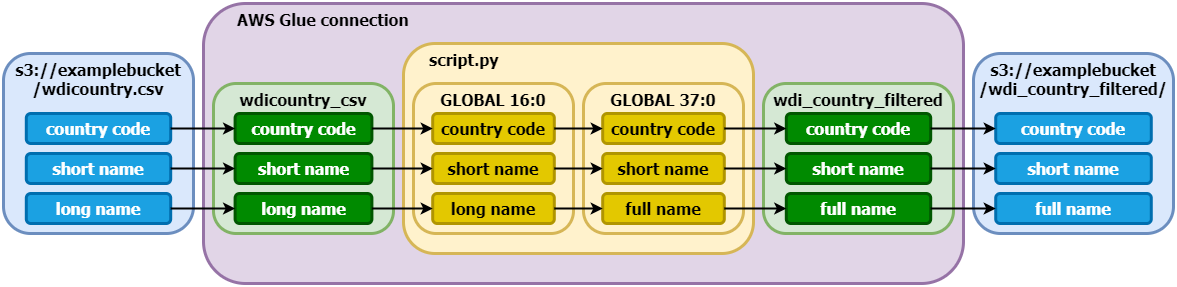
\includegraphics[width=1.0\textwidth]{img/catalog_lineage.png}
\caption{An example of data lineage graph containing Data Catalog tables}
\label{fig:catalogLineage}
\end{figure}

\section{Design of AWS Glue scanner}

The analysis from the previous section creates a strong foundation upon which we can build the design of AWS Glue scanner. We were thinking ahead when creating this design so it covers not only the features implemented in the MVP included in this work, but also the features that while not required for the purposes of the MVP, need to be implemented in near future to create a full-fledged scanner.
\par
AWS Glue scanner is designed in a standard way consisting of two main components: Connector and Dataflow Generator. The task of the Connector is to connect to AWS Glue, extract all required metadata and transform it into a general model that can be used for data flow analysis. Dataflow Generator uses this model to analyze data flows and create a data lineage graph. 

\subsection{Connection scope}
Each scenario executed in Manta Flow CLI analyzes a single connection to a data technology. The first thing we need to specify is the scope of a connection in AWS Glue, that is, what entities are analyzed in one scenario execution. Usually, this scope is defined by connection URL (where available) and credentials. A scenario then analyzes everything it has access to using these connection settings. It makes sense to use this approach in AWS Glue as well. A connection in AWS Glue scanner is defined by credentials and the AWS region. This pairing uniquely identifies the AWS Glue service instance (a service instance can be identified by an AWS account ID, which we can obtain from credentials, and by an AWS region). This connection provides access to a set of ETL jobs and Data Catalog, which together represent the connection's scope of the data flow analysis. The access can be restricted by permissions set in AWS IAM service.

\subsection{AWS Glue Connector design}
AWS Glue Connector takes care of extracting and storing metadata from AWS Glue and resolving the inputs for data flow analysis. The connector is divided into 4 main components, as is common with other scanners:
\begin{enumerate}
    \item \textit{Extractor} which extracts metadata from AWS Glue
    \item \textit{Model} which contains the definition of the general model of the input
    \item \textit{Resolver} which is an implementation of the general model
    \item \textit{Reader} which reads extracted metadata into the model used by Dataflow Generator
\end{enumerate}

\subsubsection{Extractor}
The extractor connects to the AWS Glue service instance and extracts all required metadata, saving them on the file system. To extract the metadata, AWS Java v2 SDK is used. The SDK returns data in its own Java objects. We need to extract Data Catalog metadata and ETL job metadata including job scripts. We must not forget that we also need to extract additional libraries and files which are specified in job arguments.
\par
Extracted metadata must be stored in a convenient format and in a well-defined hierarchy on the file system so that it can be correctly loaded into the model used in the data flow analysis. It is common to store metadata in the format in which it was extracted from data technology. In a situation where retrieval of a particular artifact fails (due to insufficient rights or other error), the user can provide it manually. Users can export AWS Glue metadata in multiple formats (using \texttt{aws-cli}, a command line tool for interacting with AWS services), so we chose JSON format for convenience.
\par
The file hierarchy for extracted metadata has to be unambiguous so that the Reader can read it correctly. We designed the file hierarchy shown in Figure~\ref{fig:hierarchy}. Names enclosed in \texttt{< >} represent variable names based on the actual name of the entity described between \texttt{< >} (\texttt{<job1>} would be replaced by the actual name of the first extracted ETL job etc.). The hierarchy intentionally uses \texttt{<region>} and \texttt{<account-id>} top-most directories. While a connection can only extract metadata in a single region, the name of the region is not a part of any metadata, but is required for correct naming of resources, so we store this value in the name of the directory. Account ID can be inferred from Catalog ID stored in table and database metadata, but this value is not present in job metadata and we need it to correctly resolve which Data Catalog is used in job scripts (if no Catalog ID is used when accessing Data Catalog resources, the default one is used), so we stored it in the directory name as well. However, it has another reason. It is possible to use Data Catalog belonging to another AWS account in ETL jobs, so when its metadata is extracted, it is stored in a different directory under that account's ID. Then there are two directories, \texttt{jobs} directory containing ETL job metadata and \texttt{data\_catalog} directory containing Data Catalog metadata. ETL job metadata consist of metadata JSON file and script file, if the job uses additional libraries or files, they would also be stored here. Data Catalog metadata contain JSON files of databases and tables.

\begin{figure}[ht]\centering
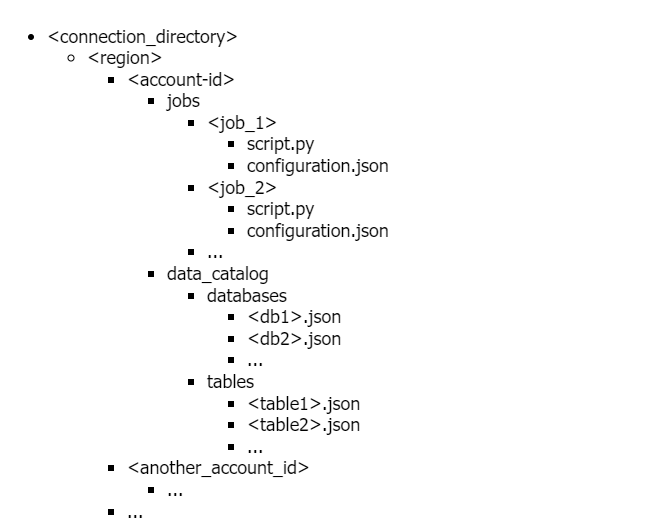
\includegraphics[width=1.0\textwidth]{img/file_hierarchy.png}
\caption{File hierarchy of extracted AWS Glue metadata}
\label{fig:hierarchy}
\end{figure}

\subsubsection{Model, Resolver and Reader}
Model component defines a common data interface of the entities of the general model of AWS Glue input following the principle of loose coupling.
\par
Resolver component contains implementations of Model interfaces. Classes are designed to be immutable so the input for the data flow analysis cannot be accidentally modified.
\par
Reader component takes care of reading the extracted metadata and creating its object representation using the classes defined in Resolver.

\subsection{AWS Glue Dataflow Generator design}

AWS Glue Dataflow Generator analyzes data flows in the extracted inputs and creates a data lineage graph. Analyzing ETL jobs is fairly simple, all that the Generator needs to do is to call Embedded Code Service. After that it merges the result graph into the AWS Glue graph containing a node representing the job and the work is done. A more interesting problem is the analysis of Data Catalog metadata.
\par
The goal of Data Catalog analysis is to create data flow edges between the nodes representing Data Catalog tables and the nodes representing the actual data sources as well as adding edges when these tables are used in ETL jobs. There are two possibilities how we can achieve that.
\par
The first approach can create a more precise data lineage, but this lineage is only created when Data Catalog is used from AWS Glue (other AWS services can also use Data Catalog, for example AWS Athena can use Data Catalog tables in SQL queries). When ETL jobs are analyzed by Embedded Code Service, the resulting graph shall contain pin nodes representing reads and writes to Data Catalog tables. Then, Dataflow Generator would create the node for this table and map the pin node to the table node. Dataflow generator would also create data source node that the table is mapped to and link it with the table node. In case of Python, table schema could be passed directly to Python analysis using Outsight to provide a more detailed column-level lineage.
\par
The second approach is a more general solution. Firstly, Data Catalog metadata would be stored in a data dictionary so it could be accessed by Dataflow Query Service. Since mapping between the data source and Data Catalog table is visualized as a data flow, it is also possible to create these flows in an extra data flow scenario. Such scenario would create data flows from data sources to Data Catalog tables for all tables present in extracted metadata. Python scanner would use Dataflow Query Service to resolve Data Catalog accesses without the need to create any extra data flows to data sources, because they would already exist. However, since there would be only dataflows from data sources to catalog tables, edges in the other direction (backlinks, when data is written to Data Catalog table) would have to be added in a postprocessing scenario.
\par
The second solution provides more value and the lineage can also be reused for other scanners, that is why we prefer it. However, it implies that several new components need to be developed, namely:
\begin{enumerate}
    \item \textit{Data dictionary mapping scenario} for mapping Data Catalog metadata into a data dictionary
    \item \textit{Data Catalog data flow scenario} for creating data flows between Data Catalog tables and their data sources
    \item Specific Dataflow Query Service implementation for AWS Glue Data Catalog
    \item Backlink mapping configuration for adding a missing edge between Data Catalog table and data source when data is written to the table
\end{enumerate}

\section{Implementation of AWS Glue scanner}
In this work we implemented the MVP of AWS Glue scanner. The goal of this MVP was not to create a full-fledged scanner, but to be able to demonstrate the functionality of Embedded Code Service. The prototype can be extended in the future following the presented design. As some of the designed features are implemented in the MVP and some are not, here is a comprehensive list that sums it up:
\begin{itemize}
    \item Implemented features
    \begin{itemize}
        \item Extraction of ETL job metadata and scripts
        \item Data flow analysis of ETL jobs
        \item Creating data lineage graph
        \item Integration with Manta Flow
        \item Configuration in Admin UI
        \item Plugin for analyzing \textit{awsglue} library function calls in Python scanner
        \item Agent for AWS Glue
    \end{itemize}
    \item Unimplemented features
    \begin{itemize}
        \item Extraction of Data Catalog metadata
        \item Extraction of additional files
        \item Data flow analysis of Data Catalog    
    \end{itemize}
\end{itemize}
\par
Let us mention interesting parts from the implementation of some of the features.

\subsection{Extraction}
AWS SDK used for metadata extraction always provides responses to requests deserialized in the form of a Java object. We have stated that we want to store metadata in a serialized JSON format. To avoid implementing serialization logic, we developed a response \textit{interceptor} (the \texttt{GlueClientExecutionInterceptor} class) that intercepts a HTTP response before it is deserialized. At this point, the body of the response contains the metadata in the desired JSON format, so we copy it and let the response be deserialized, because it is also convenient to read some of the metadata from the provided response object.
\par
We have also implemented a Manta Flow Agent specialization for AWS Glue extraction. Manta Flow Agent is an application for metadata extraction. In enterprises, it is common to limit access to certain networks for security reasons. Agent was created to allow extracting metadata from systems that are not accessible from the same network as Manta Flow Server.

\subsection{Manta Flow integration}
AWS Glue scanner is fully integrated with Manta Flow. It is released as one of so-called preview scanners which can be used only in preview mode. The scanner can be configured using Admin UI as all other scanners. The configuration includes specification of credentials and filtering expressions for ETL job names that should be included in the analysis.

\subsection{Plugin for awsglue library}
While not directly a part of AWS Glue scanner, we have developed a plugin for Python scanner that analyzes function calls in \texttt{awsglue} library. This plugin was important to be able to analyze Python code used in AWS Glue as the function calls are often present in it. We have conducted the analysis of this library in Section~\ref{sec:python}, which sums up the range of propagation modes that need to be implemented. We have implemented the functional base of the plugin that handles the extraction of this library and invocation of its propagation modes. We have also developed two propagation modes.
\par
The first propagation mode handles \texttt{create\_dynamic\_frame\_from\_options} function. This function is used to read external data specified by the options into a \texttt{DynamicFrame}. The options are key-value pairs of string values and define the connection details of the data source. The propagation of this function is implemented in  \texttt{CreateDynamicFrameFromOptionsPropagationMode}. The propagation mode works by trying to resolve the connection options in the best-effort way. We can split the options into two sets: stream connection options and database connection options. The propagation mode creates data read flow when it matches at least a part of the connection details and provides placeholder values for missing properties. If no option can be resolved, no flow is created. That is because we have no information about whether a stream or a database is accessed. This flow is wrapped in a flow representing an unknown column of a \texttt{DynamicFrame} and propagated to the target, which is the return value of the function.
\par
The other propagation mode handles the \texttt{toDF} function of \texttt{DynamicFrame} class that converts this frame into PySpark \texttt{DataFrame}. Developers often prefer PySpark frames to AWS Glue frames, because they are used to them and are more capable. First, the propagation mode \texttt{DynamicFrameToDataframePropagationMode} discovers all flows representing a column in a \texttt{DynamicFrame} and transforms them to a flow representing a \texttt{DataFrame} column, preserving column name and the source of the data in the column. Transformed flows are propagated to the target, which is the return value of the function. These flows can then be used by the plugin that handles function calls of PySpark library to resolve any function calls on the returned data frame.

 

 